\documentclass[11pt,letterpaper]{article}

\usepackage[small,compact]{titlesec}
\usepackage[margin=1in]{geometry}
\usepackage{graphicx}% http://ctan.org/pkg/graphicx
\usepackage{xcolor,colortbl}
\usepackage{enumitem}

\definecolor{Gray}{gray}{0.85}
\newcolumntype{a}{>{\columncolor{Gray}}c}

\linespread{1.45}

\title{A Comparison of Image Steganography Techniques}
\author{Neivin Mathew, Robyn Rintjema, Steven Kalapos}
\begin{document}

% Make title
\begin{titlepage}
	\maketitle
	\thispagestyle{empty}
\end{titlepage}

\clearpage
\section{Introduction}
While both cryptography and steganography provide a way to securely send messages between two parties, the difference lies in how those messages are obscured. In cryptography the plain text message is secured in cipher text, and while this may be difficult to crack it is easily identifiable as a secret message. The goal in steganography is to hide the message within other data, so that if an attacker were to stumble upon it, they would not be aware that a hidden message exists.

Through analysis of Least Significant Bit (LSB), and Discrete Cosine Transform (DCT) steganographic techniques, we hope to determine if there is a tangible difference in their performance.  The objective of this report and demonstration will be to compare these two image steganography techniques. The two implementations will be compared for effectiveness, message capacity and the impact of hiding a message on the cover image.

\section{Steganographic Algorithms}
\subsection{Least Significant Bit (LSB)}
LSB replacement is a simple steganography technique that involves swapping the least significant bit of each pixel's colour components with the bits of the message. Consequently, an image with more colour channels (RGBA, CMYK) can hide more data than those with fewer channels (RGB).
The size of the message that can be hidden in an image is:
$$capacity_{LSB} = width \times height \times |colourChannels| \ \ \ bits$$
Although the definition of LSB is confined to replacing only one bit, it can be expanded to replace two or more bits as well. Consequently, this will result in lossy modification of the pixel's colour values and degrade the image.

However, using the standard LSB algorithm will not degrade the image at all since applying it to a cover image will not modify the actual colour values as it only replaces the parity bit of each component. 

LSB is easy to detect, and is the most well known steganographic algorithm. It is also susceptible to statistical attacks making it infeasible to apply in practice. Nevertheless, it is still an effective way of concealing data.

\subsubsection{LSB Encoding}
\begin{enumerate}
\setlength\itemsep{0pt}
\item Load a copy of cover image and secret message
\item Validate that the message is small enough to fit within the cover image
\item Convert the secret message into its binary representation and prepend the length of the actual message so we know when to stop when decoding the image
\item Iterate through every pixel in the image:
\begin{enumerate}
	\setlength\itemsep{0pt}
	\item Split each pixel into its red, green and blue components
	\item Replace the Least Significant Bit of each component with a secret message bit
	\item Stop if there are no bits left to hide
\end{enumerate}
\item Write out the new image containing the secret message
\end{enumerate}

\subsubsection{LSB Decoding}
\begin{enumerate}
	\setlength\itemsep{0pt}

	\item Load the secret image and create an empty character array
	\item Create a temporary buffer that is the size of a character (depends on character encoding e.g. 8 bits)
	\item Iterate through every pixel in the image:
	\begin{enumerate}
		\setlength\itemsep{0pt}
		\item Split each pixel into its red, green and blue components
		\item Read the Least Significant Bit of each component and write it to the temporary buffer
		\item If the buffer is full, convert it to a character, write it to the message array and clear the buffer.
		\item If the character read was the special character ‘:’ that was used to delimit the message length, convert the previously read characters into the length of the message to be read
		\item If the number of characters read matches the actual length, terminate
	\end{enumerate}	
	\item Write out the extracted secret message
\end{enumerate}

\subsection{Discrete Cosine Transform}
Discrete cosine transformation depends on the DCT function:
$$ X_k = \sum_{n=0}^{N-1} x_n cos \left[ \frac{\pi}{N}\left(n+\frac{1}{2}\right)k\right]\ \ \ \ \ \ \ \ \ \ \ \  k=0,...,N-1$$

Some advantages of DCT is its robustness when it comes to image manipulation. It boasts the ability to use less bandwidth to send the image with the secret message as it can be compressed once created. However, DCT can be tricky to implement as a high degree of precision in the pixel values is needed. DCT also causes noticeable degradation in visual quality which may alert attackers to the presence of a secret message. 

Additionally, because of the need to use 8x8 blocks of pixels to store message data, the DCT message size is severely limited. The size of the message that can be hidden in an image is:
$$capacity_{DCT} = \frac{width \times height}{8 \times 8} \ \ \ bits$$

\subsubsection{DCT Encoding}
\begin{enumerate}
\setlength\itemsep{0pt}
\item Get the cover image path and secret message
\item Load in the cover image
\item Convert secret message to binary representation and add the length of the message in characters to the beginning in the form: \texttt{length*message}
\item Split the image into red, blue and green colour channels
\item Working with only the blue channel. Break the image into 8x8 blocks of pixels
\item Subtract 128 from each block to normalize pixel values around 0
\item Run each block through DCT function
\item Divide each block by the quantization table given below
\item The DC coefficient is located in position [0][0] of each pixel block and is an average of the entire block. Retrieve the DC coefficient and replace the least significant bit with the corresponding message bit
\item Multiply the image blocks by the quantization table and add 128 to each block
\item Piece together 8x8 blocks of the new image
\item Merge the new blue channel with the existing red and green channels
\item Write out the new image containing the secret message
\end{enumerate}

\subsubsection{DCT Decoding}
\begin{enumerate}
\setlength\itemsep{0pt}
\item Get the secret image and load it in
\item Split the image into red, green and blue channels (message hidden in blue channel)
\item Break the blue channel into 8x8 blocks of pixels and subtract 128 from each block
\item Divide each block by the quantization table above
\item Read in the least significant bit of each DC coefficient in 8 bit blocks
\item Once ‘*’ is encountered set message size to integer that came before separator
\item Read in 8 bit blocks from image, converting them to plain text characters, until the length of the message matches the message size recovered
\item Return the decoded message
\end{enumerate}

\section{Testing Methods}
To compare LSB and DCT, a standard PNG-24 image \texttt{lenna.png} sized 240x240 was used. All experiments were run on a standard 2014 Macbook Pro. The two techniques were compared in the following categories:
\begin{enumerate}
\setlength\itemsep{0pt}
\item \textbf{Time Taken} -- The time taken to encode the same \texttt{10kB} plaintext message into our image was recorded and compared.

\item \textbf{Message Size} -- The maximum limit for size of the message that could be hidden within the standard image was analyzed.

\item \textbf{Visual Quality} -- A qualitative analysis of the visual quality of the image was also conducted. 

\item \textbf{Image Error} -- The following measures of image error were used to compare the two techniques.
\begin{itemize}
\setlength\itemsep{0pt}
\item \textbf{Mean Squared Error (MSE)}

The MSE between the encoded image and the original image was calculated using the below equation. An MSE of zero means less image deviation from original, while an MSE of more than 1 indicates less similarity (grows as the differences in pixel colours increases.
$$MSE = \frac{1}{MN}\sum_{n=1}^{M}\sum_{m=1}^{N} \left[\ h(n,m) - g(n,m) \right]^2 \ \ \ \ for\ images\ g(n,m)\ and\ h(n,m)$$

\item \textbf{Structural Similarity Index (SSIM)}

The structural similarity index(SSIM) is used to measure similarity between two images based on their luminance, contrast and structure. A SSIM value of 1 means there is no perceived difference in the images. The measure between two windows $x$ and $y$ of common size $N \times N$ is:
$$
SSIM(x,y) = \frac{(2\mu_x\mu_y + c_1)(2\sigma_xy + c_2)}{(\mu_x^2 + \mu_y^2 + c_1)(\sigma_x^2 + \sigma_y^2 + c_2)}
$$
where $\mu_x$ is the average of $x$\\
$\mu_y$ is the average of $y$\\
$\sigma_x^2$ is the variance of $x$\\
$\sigma_y^2$ is the variance of $y$\\
$\sigma_xy$ is the covariance of $x$ and $y$\\
$c_1=(k_1L)^2, c_2=(k_2L)^2$ used as variables to stabilize division with weak denominator\\
$L$ is the dynamic range of pixel values\\
$k_1=0.01$ and $k_2=0.03$ by default
\end{itemize}
\end{enumerate}

\section{Results}
\begin{center}
{\renewcommand{\arraystretch}{1.4}% for the vertical padding
\begin{tabular}{ a|c|c|c }
	\hline
	Result & Original & LSB & DCT \\
 Image & 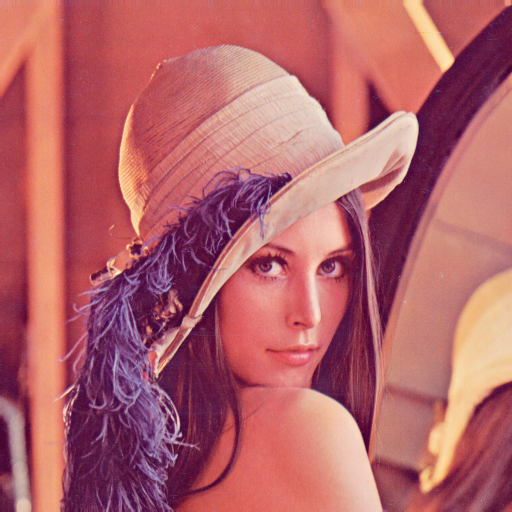
\includegraphics[width=40mm]{lenna.png} & 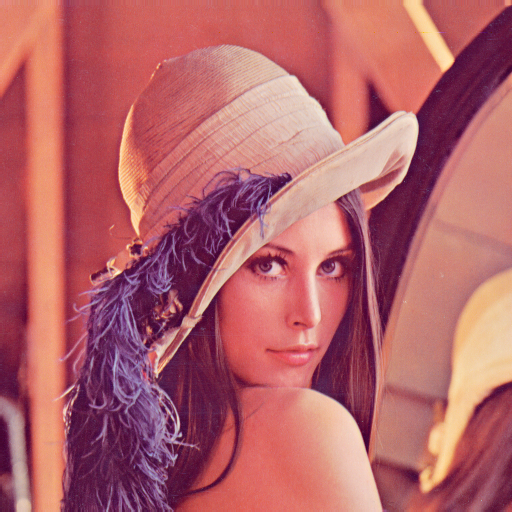
\includegraphics[width=40mm]{LSBlenna.png} & 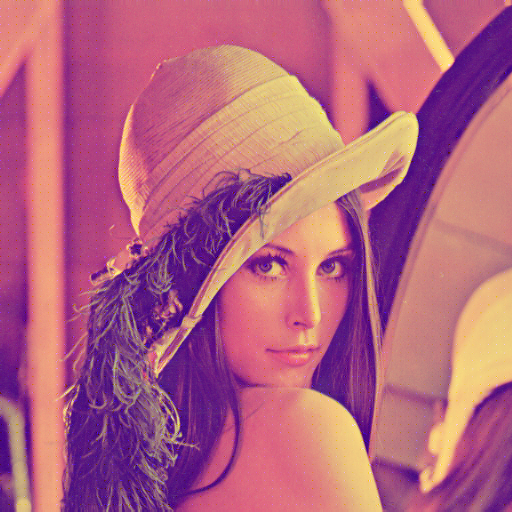
\includegraphics[width=40mm]{DCTlenna.png} \\ 
 Time Taken & N/A & {\renewcommand{\arraystretch}{0.9}\begin{tabular}{@{}c@{}}Encoding: 0.171s \\ Decoding: 0.031s \end{tabular}} & {\renewcommand{\arraystretch}{0.9}\begin{tabular}{@{}c@{}}Encoding: 0.234s \\ Decoding: 0.075s \end{tabular}}\\  
 Message Size& N/A & 21,600 bytes & 450 bytes\\
 Visual Quality&N/A& No quality difference & {\renewcommand{\arraystretch}{0.9}\begin{tabular}{@{}c@{}}Slight blue tint\\ Grid pattern present\end{tabular}}\\
 MSE& 0.0 &0.02&1,886.86\\
 SSIM&1.0&0.98&0.76\\
\end{tabular}
}
\end{center}

\section{Conclusion}
Both algorithms allowed for effective embedding and retrieval of the test message. Based on the results it can be concluded that the LSB algorithm provides a better image quality after embedding. This can be seen through analysis of the MSE and SSIM values as well as a visual inspection of the images. The time taken to encrypt and decrypt also favoured LSB, however the difference was negligible in a real world setting. However, LSB provides less security against attacks if the image is recognized as a steganographic image.

\clearpage
\section{Tools Used}
The project was implemented in Python and utilized the following libraries:
\begin{itemize}
\setlength\itemsep{0pt}
\item OpenCV
\item Pillow (Python Imaging Library)
\item SciKit-Image
\item NumPy
\item Matplotlib
\end{itemize}

\section{Bibliography}
\begin{enumerate}[label={[\arabic*]}]
\item M. Sravanthi, M. Devi, S. Riyazoddin, and M. Reddy, “A Spatial Domain Image Steganography Technique Based on Plane Bit Substitution Method,” Glob. J. Comput. …, vol. 12, no. 15, 2012.
\item S. Dhall, B. Bhushan, and S. Gupta, “An in-depth analysis of various steganography techniques,” Int. J. Secur. its Appl., vol. 9, no. 8, pp. 67–94, 2015.
\item F. M. Shelke, A. A. Dongre, and P. D. Soni, “Comparison of different techniques for Steganography in images,” vol. 3, no. 2, pp. 171–176, 2014.
\item G. Kaur and A. Kochhar, “A Steganography Implementation based on LSB \& DCT,” vol. 4, no. 1, pp. 35–41, 2012.
\end{enumerate}



\end{document}
